
\section{Standard Slides}\label{sec:standard-slides}

\subsection{Text Only}\label{ssec:text-only}

\begin{frame}
	\frametitle{Default Text Slide}
	%Content goes here
	Vero minima pariatur ea itaque natus in. In quidem non error fugiat tempore aliquid magni. Animi aliquam voluptatum eum. Delectus voluptate illum quidem et autem.
\end{frame}

\subsection{Lists}\label{ssec:lists}

\begin{frame}
	\frametitle{Itemize and Listing}
	%Content goes here
	Vero minima pariatur ea itaque natus in. In quidem non error fugiat tempore aliquid magni. Animi aliquam voluptatum eum.
	\pause
	 Delectus voluptate illum quidem et autem.

	\begin{itemize}[<+->]
		\item This one is always shown
		\item The first time (i.e. as soon as the slide loads)
		\item The second time
		\item Also the first time
		\only {This one is shown at the first time, but it will hide soon (on the next event after the slide loads).}
	\end{itemize}
\end{frame}

\subsection{Graphics}\label{ssec:graphics}

\frame[plain]{
	\frametitle{Include an Image}
	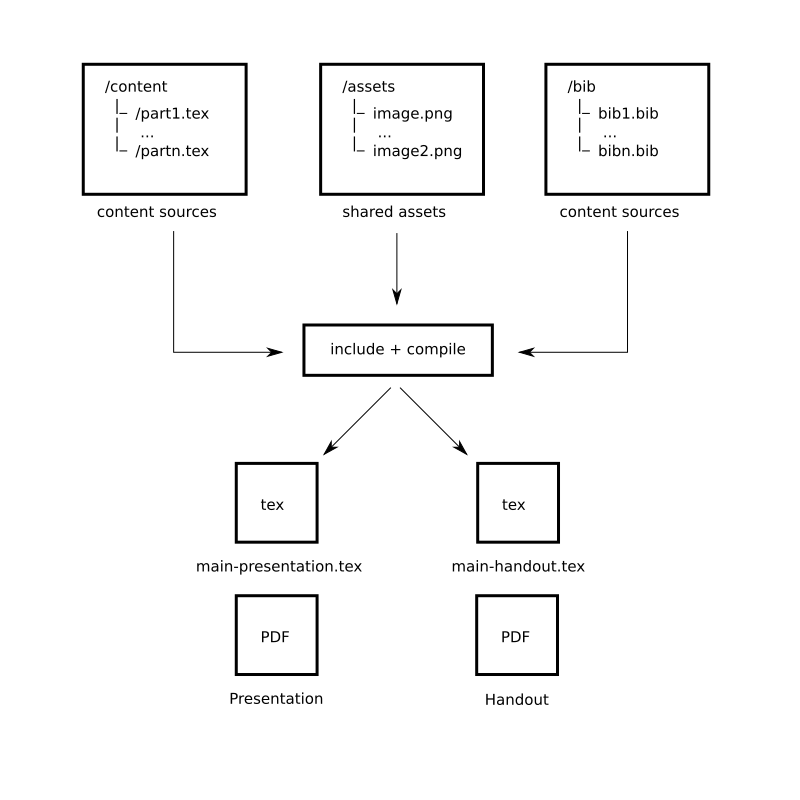
\includegraphics[width=0.5\linewidth]{./assets/overview.png}
}

\section{Include Source Code}\label{sec:include-source-code}

\begin{frame}[fragile]
\frametitle{Some Simple C Code}

\begin{lstlisting}[caption=Some JavaScript code,label={lst:lstlisting}]
var x = 3;
var y = 5;

this.bla;
var obj = new Object();

/**
 * Adds to variables and returns the result.
 **/
obj.add = function(a, b) {
	return a + b;
};

var z = obj.add(x, y);

console.log("bla");

\end{lstlisting}
\end{frame}

\section{Columns on Slides}\label{sec:columns-on-slides}

\begin{frame}
	\frametitle{Example of columns 2}
	\begin{columns}[T] % contents are top vertically aligned
	\begin{column}[T]{5cm} % each column can also be its own environment
	Contents of first column \\ split into two lines \\
	Pagenumbers: \insertframenumber/\inserttotalframenumber
	\end{column}
	\begin{column}[T]{5cm} % alternative top-align that's better for graphics
          		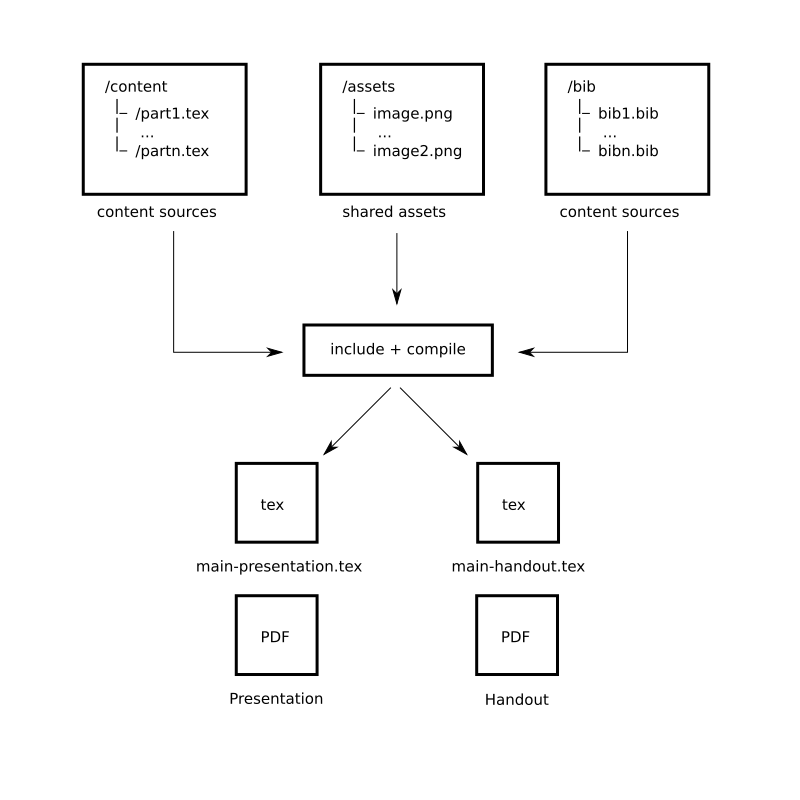
\includegraphics[height=3cm]{./assets/overview.png}
	\end{column}
	\end{columns}
\end{frame}


\section{Blocks on Slides}\label{sec:blocks-on-slides}


\begin{frame}

   \begin{block}{This is a Block}
      This is important information
   \end{block}

   \begin{alertblock}{This is an Alert block}
   This is an important alert
   \end{alertblock}

   \begin{exampleblock}{This is an Example block}
   This is an example
   \end{exampleblock}

\end{frame}
